% Created 2023-08-25 Fri 16:52
% Intended LaTeX compiler: pdflatex
\documentclass[11pt,a4paper,final]{article}
\usepackage[a4paper, total={7in, 10in}]{geometry}
\usepackage{algorithm2e}
\usepackage{booktabs}
\usepackage{subcaption}
\usepackage{graphicx}
\usepackage{tikz}
\usepackage[utf8]{inputenc}
\usepackage[T1]{fontenc}
\usepackage{graphicx}
\usepackage{longtable}
\usepackage{wrapfig}
\usepackage{rotating}
\usepackage[normalem]{ulem}
\usepackage{amsmath}
\usepackage{amssymb}
\usepackage{capt-of}
\usepackage{hyperref}
\usepackage[T1]{fontenc}
\usepackage{lmodern}
%%==============================================================================
% Package configuration
\usepackage{amsmath}                                  % Miscellaneous enhancements for mathematics
\usepackage{amssymb}                                  % Math symbols
\usepackage{booktabs}                                 % Extend tables
\usepackage{cite}                                     % Improved citation mechanics
\usepackage{graphicx}                                 % Enhance graphics
\usepackage{lineno}                                   % Add line numbers to page
\usepackage{microtype}                                % Uses different techniques for spacing
\usepackage{multicol}                                 % Create tables spanning multiple columns
\usepackage{multirow}                                 % Create tables spanning multiple rows
\usepackage{pgfplots}                                 % Plot in LaTeX
\usepackage{subcaption}                               % Subfigures (Get rid of this)
\usepackage{subfloat}                                 % Subfigures
\usepackage{tabularx}                                 % Add more contol to tables
\usepackage{tikz}                                     % Generate figures in LaTeX
\usepackage{xcolor}                                   % Colors
\usepackage{xfp}                                      % No trailing zeros
\usepackage{standalone}                               % Include standalone documents
\usepackage{hyperref}                                 % Better references (keep last)
%% Plot configurations
\usetikzlibrary{automata, positioning, arrows.meta}   % Tikz macros
\pgfplotsset{compat=1.3, width=\textwidth}
\graphicspath{ {img} }                                % Paths to find images
%% Paper configuration
\let\ref\autoref                                      % Redifine `\ref` as `\autoref` because lazy
%%==============================================================================
% `autoref' formatting
\renewcommand*{\sectionautorefname}{Section}
\renewcommand*{\subsectionautorefname}{Subsection}
\renewcommand*{\subsubsectionautorefname}{Subsubsection}
\renewcommand*{\paragraphautorefname}{Paragraph}
%%===============================================================================
% Custom Commands
\newcommand{\TODO}[1]{{\color{green} To do: #1}}                                % For adding notes to paper
%%-------------------------------------------------------------------------------
% Experiment parameters
% TODO: Ensure these are accurate
\newcommand{\A}{35 }                                                            % Number of buses
\newcommand{\N}{338 }                                                           % Number of visits
\newcommand{\acharge}{0.9}                                                      % BOD charge percentage
\newcommand{\bcharge}{0.7 }                                                     % EOD charge percentage
\newcommand{\mincharge}{25\% }                                                  % Min visit charge percent
\newcommand{\minchargeD}{0.25 }                                                 % Min visit charge decimal
\newcommand{\maxcharge}{100\% }                                                 % Max visit charge percent
\newcommand{\batsize}{388 }                                                     % Battery capacity
\newcommand{\fast}{15 }                                                         % Number of fast chargers
\newcommand{\slow}{15 }                                                         % Number of slow chargers
\newcommand{\fasts}{911 }                                                       % Speed of fast charger
\newcommand{\slows}{30 }                                                        % Speed of slow charger
\newcommand{\contvars}{7,511 }
\newcommand{\intvars}{328,282 }
%%-------------------------------------------------------------------------------
%% Solve output
\newcommand{\timeran}{1800 }                                                    % Time ran for MILP [s]
\newcommand{\gappercent}{65.2\% }                                               % Gap percent after runtime
\newcommand{\processor}{Ryzen 9 }                                               % Processor type
\newtheorem{definition}{Definition}[section]
\author{Alexander Brown}
\date{\today}
\title{Fuzzy Bus Charging Schedule With MILP Constraints}
\hypersetup{
 pdfauthor={Alexander Brown},
 pdftitle={Fuzzy Bus Charging Schedule With MILP Constraints},
 pdfkeywords={},
 pdfsubject={},
 pdfcreator={Emacs 29.1 (Org mode 9.6.7)}, 
 pdflang={English}}
\begin{document}

\maketitle
\tableofcontents

\let\ref\autoref                            % Redifine `\ref` as `\autoref` because lazy

\section{Introduction}
\label{sec:orgac4f960}
This document outlines a fuzzy model of the Position Allocation Problem (PAP). The model utilizes Mixed Integer Linear
Programming (MILP) constraints to determine feasible charging schedules. The problem involves generating an optimal
charging schedule for a fleet of Battery Electric Buses (BEBs) based on a set of routes and a mix of fast and slow
chargers. The objective is to reduce the number of total chargers and reduce the amount of time spent charging. The
samples utilized are a subset of the UTA bus routes from which the route times and time spent at the station are derived.
This paper assumes an average discharge over a period from which an estimated discharge is calculated for each route,
\(\Delta_i\). Furthermore, linear battery dynamics are also assumed. Linear battery dynamics are a valid assumption when the
state-of-charge (SOC) is below 80\% charge \cite{liu-2020-batter-elect}.

The Fuzzy PAP (FPAP) expands upon the MILP-PAP by adding a layer of robustness to the model's solutions
\cite{bello-2019-fuzzy-activ,kaur-2016-introd-fuzzy}. By introducing fuzziness to the model, that allows a sense of
uncertainty to some of the parameters. In a realistic scenario, multiple factors such as technical problems, weather
conditions, road detours, among others, buses may arrive earlier or later than anticipated to the station/depot. For
crisp models, there is no sense of lateness or earliness, thus the model's solutions lose validity at the moment that
any buses do not adhere to the route time perfectly. Fuzzifying the models in turn produces a fuzzy solution that
encodes ranges of times that buses may arrive while still remaining a valid solution.

The paper proceeds as follows. \ref{sec:preliminaries} introduces some of the basic concepts of Mixed Integer Linear
Programming (MILP), fuzzy set theory, and Fully Fuzzy Linear Programming (FFLP). \ref{sec:the-crisp-bap-and-pap} introduces
the Berth Allocation Problem (BAP) from which the PAP and MILP-PAP are derived from. The MILP-PAP is also derived in
full. \ref{sec:the-fuzzy-bap} introduces and derives a Fuzzy BAP (FBAP) model. \ref{sec:the-fuzzy-pap} then adapts the PAP into
the FPAP by utilizing the results from the previous sections.
\section{Preliminaries}
\label{sec:preliminaries}
\subsection{Mixed Integer Linear Program}
\label{sec:org2bd898b}
A mixed integer linear programming (MILP) problem is a class of constrained optimization in which one seeks to find a
set of continuous or integer values that maximizes or minimizes an objective function while satisfying a set of
constraints \cite{chen-2010-applied}. Given a general objective function \(J\), decision variables (i.e. variables of
optimization) \(x_j \in \mathbb{R}\) and \(y_k \in \mathbb{Z}^+\), and input parameters \(c_j, d_k, a_{ij}, g_{ik}, b_i \in \mathbb{R}\), a MILP has the
mathematical structure represented in \ref{eq:milp-structure} \cite{chen-2010-applied}.

\begin{equation}
\label{eq:milp-structure}
\begin{array}{lll}
\text{max}   & J = \sum_j c_j x_j + \sum_k d_k y_k            &                 \\
\text{subject to} & \sum_j a_{ij} x_j + \sum_k g_{ik} y_k  \le b_i & (i = 1,2,...,m) \\
                  & x_j \ge 0                                      & (j = 1,2,...,n) \\
                  & y_k \in \mathbb{Z^+}0                          & (k = 1,2,...,n) \\
\end{array}
\end{equation}

This formulation of the MILP is also referred to as ``crisp''. By this it is meant that each variable in the formulation
acts as an injective mapping to its number representation. In other words, every variable has a one-to-one mapping from
variable to value \cite{kaur-2016-introd-fuzzy}.

\subsection{Fuzzy Sets Theory}
\label{sec:org36b8442}
This section introduces the notion of fuzzy numbers and some basic definitions. Concepts from this section are pulled
from \cite{zimmermann-2001-fuzzy-set,das-2016-mathem-model,yaghobi-2014-compar-fuzzy,bello-2019-fuzzy-activ}.

\subsubsection{Fuzzy Sets}
\label{sec:orgae38a69}
Let's begin with what a fuzzy number is not. A classical (crisp) set is defined as a collection of elements \(x \in X\).
Crisp sets are binary, either an element belongs in the set, or it does not \cite{zimmermann-2001-fuzzy-set}. For a
fuzzy set, what is known as the characteristic function applies various degrees of membership for elements of a given
set \cite{zimmermann-2001-fuzzy-set}.

\begin{definition}
Let \(X\) be a collection of objects (often called the universe of discourse \cite{bello-2019-fuzzy-activ}). If \(X\) is denoted
generically by \(x\), then a fuzzy set \(\tilde{A}\) in \(X\) is a set of ordered pairs as shown in \ref{eq:membership-function}.

\begin{equation}
\label{eq:membership-function}
\tilde{A} = \{(x, \mu_{\tilde{A}}(x))| x\in X\}
\end{equation}

\noindent
\(\mu_{\tilde{A}}\) is called the membership function where \(\mu_{\tilde{A}}\) is the mapping \(\mu_{\tilde{A}} : X \rightarrow
[0,1]\); which assigns a real number to the interval \([0,1]\). The value of \(\mu_{\tilde{A}}\) represents the degree of
membership of \(x\) in \(\tilde{A}\).
\end{definition}

This paper will use fuzzy sets defined over the set of real numbers \(\mathbb{R}\). There are multiple ways to represent fuzzy
numbers over the set of real numbers. The representation is defined by membership function which describes the shape of
the fuzzy number. As an example, consider the following definition.

\begin{definition}
A fuzzy number that is represented by \(\tilde{A} = (a,b,c)\) is said to be triangular if its membership function is
defined as \ref{eq:triangular-fuzzy-number}.

\begin{equation}
\label{eq:triangular-fuzzy-number}
  \mu_{\tilde{A}}(x) =
  \begin{cases}
    \frac{(x-a)}{(b-a)} & a \le x \le b \\
    \frac{(d-x)}{(d-b)} & c \le x \le d \\
    0                   & \text{otherwise}
  \end{cases}
\end{equation}
\end{definition}

\begin{definition}
The fuzzy set \(\tilde{A}\) in \(\mathbb{R}\) is normal if \(\text{max}_x \mu_{\tilde{A}}(x) = 1\).
\end{definition}

\begin{definition}
A fuzzy set \(\tilde{A}\) in \(\mathbb{R}\) is convex if and only if the membership function of \(\tilde{A}\) satisfies the inequality

\begin{equation*}
\mu_{\tilde{A}}[\beta x_1 + (1-\beta)x_2] \ge \text{min}[\mu_{\tilde{A}}(x_1), \mu_{\tilde{A}}(x_2)]\; \forall x_1, x_2 \in \mathbb{R}\; \beta \in [0,1]
\end{equation*}
\end{definition}

\begin{definition}
A fuzzy number is a normal convex fuzzy set in \(\mathbb{R}\).
\end{definition}

\begin{definition}
The triangular fuzzy number \(\tilde{A}\) is nonnegative \(\iff\; a \ge 0\).
\end{definition}

A more general definition of fuzzy numbers is known as LR fuzzy numbers
\cite{kaur-2016-introd-fuzzy,zimmermann-2001-fuzzy-set}.

\begin{definition}
A function \(L:[0,\infty] \rightarrow [0,1]\) (or \(R:[0,\infty] \rightarrow [0,1]\)) is said to be reference a function of the fuzzy number if and only
if

\begin{enumerate}
\item \(L(0) = 1\) (or \(R(0) = 1\))
\item \(L\) (or \(R\)) is non-increasing on \([0,\infty)\)
\end{enumerate}
\end{definition}

\begin{definition}
A fuzzy number \(\tilde{A}\) defined on the set of real numbers, \(\mathbb{R}\), denoted as \((m,n,\alpha,\beta)_{LR}\), is said to be an \(LR\)
flat fuzzy number if its membership function \(\mu_{\tilde{A}}(x)\) is defined as

\begin{equation}
\mu_{\tilde{A}}(x) =
\begin{cases}
L(\frac{m-x}{\alpha}) & x \le m, \alpha > 0 \\
R(\frac{m-n}{\beta}) & x \ge m, \beta > 0 \\
1                & m \le x \le n
\end{cases}
\end{equation}
\end{definition}

\begin{definition}
An \(LR\) flat fuzzy number \(\tilde{A} = (m,n,\alpha,\beta)_{LR}\) is said to be a non-negative \(LR\) flat fuzzy number if and only
if \(m-\alpha \ge 0\) and is said to be non-positive \(LR\) flat fuzzy number if and only if \(m - \alpha \le 0\) is a real number.
\end{definition}

\begin{definition}
An \(LR\) flat fuzzy number \(\tilde{A} = (m,n,\alpha,\beta)_{LR}\) is said to be an unrestricted \(LR\) flat fuzzy number if and only
if \(m - \alpha\) is a real number.
\end{definition}

\subsubsection{Fuzzy Arithmetic}
\label{sec:org30e0199}
If two triangular fuzzy numbers \(\tilde{a}_1 = \{a_1, a_2, a_3\}\) and \(\tilde{b}_1 = \{b_1, b_2, b_3\}\) are nonnegative
then the following operations are defined in \ref{eq:fuzzy-arithmetic}.

\begin{equation}
\label{eq:fuzzy-arithmetic}
\begin{array}{lcl}
\tilde{a} \oplus \tilde{b} & = & (a_1 + b_1, a_2 + b_2, a_3 + b_3) \\
\tilde{a} \ominus \tilde{b} & = & (a_1 + b_3, a_2 + b_2, a_3 + b_1) \\
\tilde{a} \otimes \tilde{b} & = & (a_1 b_1, a_2 b_2, a_3 b_3)       \\
\end{array}
\end{equation}

\subsubsection{Comparing Fuzzy Numbers}
\label{sec:orga6c4bcc}
Fuzzy numbers do not directly provide a method of ordering nor do they always provide an ordered set like real numbers
\cite{bello-2019-fuzzy-activ}. There are multiple methods for ordering fuzzy numbers, each coming with advantages and
disadvantages. Different properties have been applied to justify comparison of fuzzy numbers, such as: preference,
rationality, and robustness \cite{jimenez-2007-linear-progr,bello-2019-fuzzy-activ,kaur-2016-introd-fuzzy}. These
methods are commonly known as ranking functions or ordering functions
\cite{bello-2019-fuzzy-activ,das-2016-mathem-model,kaur-2016-introd-fuzzy}. Commonly, including in this work, the First
index of Yager \cite{yager-1981-proced-order} is used (\ref{eq:first-index-yager}).

\begin{equation}
\label{eq:first-index-yager}
\mathfrak{R}(\tilde{A}) = \frac{\sum_i a_i}{|\tilde{A}|}
\end{equation}

\noindent where \(|\cdot|\) represents the cardinality of the fuzzy number. In words, \ref{eq:first-index-yager} is merely the
average of the values in the fuzzy number. As a result, \(A \le B\) when \(\mathfrak{R}(\tilde{A}) \le \mathfrak{R}(\tilde{B})\)
\cite{bello-2019-fuzzy-activ}.

\subsection{Fully Fuzzy Linear Programming}
\label{sec:fully-fuzzy-linear-programming}
Much like the MILP, Fully Fuzzy Linear Programs (FFLP), it is a class of constrained optimization in which one seeks to
find a set of continuous variables that either maximizes or minimizes an objective function, \(J\), while satisfying a set
of constraints. The key difference in FFLP is that it is designed to accommodate imprecise information
\cite{bello-2019-fuzzy-activ,kaur-2016-introd-fuzzy}. In FFLP, the parameters and decision variables are fuzzy and
linear. A general FFLP is represented as shown in \ref{eq:general-fflp}. The subscripts \(\cdot_e\), \(\cdot_l\), and \(\cdot_g\) indicate to
equality, less than, and greater than constraints, respectively.

\begin{equation}
\label{eq:general-fflp}
\begin{array}{lll}
\text{max}   & J = \sum_j \tilde{C}_j \otimes \tilde{X}_j              &                 \\
\text{subject to} & \sum_j \tilde{a}_{ej} \otimes \tilde{x}_j = \tilde{b}_e &  \forall e = 1,2,3,... \\
                  & \sum_j \tilde{a}_{lj} \otimes \tilde{x}_j \le \tilde{b}_l &  \forall l = 1,2,3,... \\
                  & \sum_j \tilde{a}_{gj} \otimes \tilde{x}_j \ge \tilde{b}_l &  \forall g = 1,2,3,...
\end{array}
\end{equation}

There are many methods of solving FFLP
\cite{bello-2019-fuzzy-activ,kaur-2016-introd-fuzzy,ebrahimnejad-2016-new-method,nasseri-2013-fully}; however, the
general strategy is to convert the fuzzy model into a crisp model that can be solved using traditional methods
\cite{bello-2019-fuzzy-activ}. In \cite{nasseri-2013-fully,bello-2019-fuzzy-activ}, the method of converting the FFLP
into a crisp MILP is simply done by applying the ranking function to the objective function and breaking the constraints
down into a set of crisp constraints as shown in \ref{eq:nasseri-solution}. The constraints are separated according to the
definition of fuzzy set multiplication defined in \ref{eq:fuzzy-arithmetic}. The fuzzy number index is represented is the
exponent rather than the subscript to clearly distinguish between the indexed value in the fuzzy number and the
constraint index (i.e. \(\tilde{A} = (a^1,a^2,a^3)\)). Furthermore, it is assumed that the fuzzy numbers are nonnegative.
Although the following equation can be written in terms of general nonnegative LR fuzzy numbers, the parameters and
decision variables are written in terms of nonnegative triangular fuzzy numbers.

\begin{equation}
\label{eq:nasseri-solution}
\begin{array}{lclc}
\text{max}   & J = \mathfrak{R}\Big(\sum_j (c_j^1,c_j^2,c_j^3)(x_j^1,x_j^2,x_j^3)\Big) &\\
\text{subject to} & \sum_j a_{ej}^1 x_j^1 = b_e^1 & & \forall e = 1,2,3,... \\
                  & \sum_j a_{lj}^1 x_j^1 \le b_l^1 & & \forall l = 1,2,3,... \\
                  & \sum_j a_{gj}^1 x_j^1 \ge b_g^1  & & \forall g = 1,2,3,... \\
                  & \sum_j a_{ej}^2 x_j^2 = b_e^2 & & \forall e = 1,2,3,... \\
                  & \sum_j a_{lj}^2 x_j^2 \le b_l^2 & & \forall l = 1,2,3,... \\
                  & \sum_j a_{gj}^2 x_j^2 \ge b_g^2  & & \forall g = 1,2,3,... \\
                  & \sum_j a_{ej}^3 x_j^3 = b_e^3 & & \forall e = 1,2,3,... \\
                  & \sum_j a_{lj}^3 x_j^3 \le b_l^3 & & \forall l = 1,2,3,... \\
                  & \sum_j a_{gj}^3 x_j^3 \ge b_g^3  & & \forall g = 1,2,3,... \\
                  & x_j^2 - x_j^1 \ge 0         & x_j^3 - x_j^2 \ge 0 & \\
\end{array}
\end{equation}

\noindent Note the last constraint is defined to ensure the ordering of the triangular fuzzy number, \(x_j^1 \le x_j^2 \le x_j^3\).
To be more succinct, the FFLP can also equivalently be written as \ref{eq:nasseri-solution-condensed}.

\begin{equation}
\label{eq:nasseri-solution-condensed}
\begin{array}{llc}
\text{max}   & J = \mathfrak{R}\Big(\sum_j (c_j^1,c_j^2,c_j^3) \otimes (x_j^1,x_j^2,x_j^3)\Big) &\\
\text{subject to} & \sum_j a_{ej}^k x_j^k = b_e^k &  \forall e = 1,2,3,... \\
                  & \sum_j a_{lj}^k x_j^k \le b_l^k &  \forall l = 1,2,3,... \\
                  & \sum_j a_{gj}^k x_j^k \ge b_g^k  &  \forall g = 1,2,3,... \\
                  & x_j^2 - x_j^1 \ge 0         & x_j^3 - x_j^2 \ge 0 \\
                  & \forall k \in \{1,2,...\}        &                  \\
\end{array}
\end{equation}

Where \(k\) has a max value equal to the cardinality to the type of fuzzy number being utilized. This can be further be
elaborated on by rewriting the inequality constraints as equality constraints by introducing slack variables. This is
useful as it represents the formulation in a standard form \cite{chen-2010-applied,vanderbei-2020-linear-progr}.

The given method is called the Kumar and Kaurs method \cite{kaur-2016-introd-fuzzy} which is similar in presentation of
the Nassiri method presented in \cite{bello-2019-fuzzy-activ}. Generally speaking, it is designed to solve FFLP
problems with inequality constraints having LR flat fuzzy numbers. Given the FFLP \ref{eq:general-fflp} and assuming that
\(\tilde{x}_j\) is an LR flat fuzzy number, the problem can be reformulated as \ref{eq:kumar-kaurs-fuzzy}
\cite{kaur-2016-introd-fuzzy}.

\begin{equation}
\label{eq:kumar-kaurs-fuzzy}
\begin{array}{lll}
\text{max}   & J = \sum_j \tilde{C}_j \otimes \tilde{X}_j              &                                              \\
\text{subject to} & \sum_j \tilde{a}_{ej} \otimes \tilde{x}_j               = \tilde{b}_e & \forall e = 1,2,3,...                \\
                  & \sum_j \tilde{a}_{lj} \otimes \tilde{x}_j \oplus \tilde{S}_l = \tilde{b}_l \oplus \tilde{S'}_l & \forall l = 1,2,3,... \\
                  & \sum_j \tilde{a}_{gj} \otimes \tilde{x}_j \oplus \tilde{S}_g = \tilde{b}_g \oplus \tilde{S'}_g & \forall g = 1,2,3,... \\
                  & \mathfrak{R}(\tilde{S_l}) - \mathfrak{R}(\tilde{S_l'}) \ge 0                                     & \forall l = 1,2,3,...      \\
                  & \mathfrak{R}(\tilde{S_g}) - \mathfrak{R}(\tilde{S_g'}) \le 0                                     & \forall g = 1,2,3,...
\end{array}
\end{equation}

Expanding the set of equations and using the condensed notation in \ref{eq:nasseri-solution-condensed} we find
\ref{eq:kumar-kaurs-crisp} \cite{kaur-2016-introd-fuzzy}.

\begin{equation}
\label{eq:kumar-kaurs-crisp}
\begin{array}{lllc}
\text{max}    & J = \mathfrak{R}\Big(\sum_j (c_j^1,c_j^2,c_j^3) \otimes (x_j^1,x_j^2,x_j^3)\Big) &                             &                                          \\
\text{subject to}  & \sum_j a_{ej}^k x_j^k = b_e^k                                &                                &   \forall e = 1,2,3,...        \\
                   & \sum_j a_{lj}^k x_j^k s_l^k \le s_l^{'k} b_l^k                 &                                &   \forall l = 1,2,3,...       \\
                   & \sum_j a_{gj}^k x_j^k s_g^k \ge s_l^{'k} b_l^k                 &                                &   \forall g = 1,2,3,...      \\
                   & \mathfrak{R}(\tilde{S_l}) - \mathfrak{R}(\tilde{S_l'}) = 0                      &                                &  \forall l = 1,2,3,...          \\
                   & \mathfrak{R}(\tilde{S_g}) - \mathfrak{R}(\tilde{S_g'}) = 0                      &                                &  \forall g = 1,2,3,...          \\
                   & x_j^2 - x_j^1 \ge 0                                              &x_j^3 - x_j^2 \ge 0 &         \\
                   & s_j^2 - s_j^1 \ge 0                                              &s_j^3 - s_j^2 \ge 0 &         \\
                   & s_j^{'2} - s_j^{'1} \ge 0                                        &s_j^{'3} - s_j^{'2} \ge 0 & \\
                   & \forall k \in \{1,2,...\}                                            &                            &                       \\
\end{array}
\end{equation}
\section{The Crisp BAP and PAP}
\label{sec:the-crisp-bap-and-pap}
\subsection{The Position Allocation Problem}
\label{sec:the-position-allocation-problem}
This section provides a brief overview of the BAP and a detailed formulation of PAP as presented in
\cite{qarebagh-2019-optim-sched}.

\subsubsection{Overview of BAP}
\label{sec:overview-of-bap}
The BAP is a rectangle packing problem where a set of rectangles, \(\mathbb{O}\), are attempted to be optimally placed in
a larger rectangle, \(O\), as shown in \autoref{fig:packexample}. The rectangle packing problem is an NP-hard problem that
can be used to describe many real life problems \cite{bruin-2013-rectan-packin,murata-1995-rectan}. In some of these
problems, the dimensions of \(\mathbb{O}\) are held constant such as in the problem of packing modules on a chip, where
the widths and height of the rectangles represent the physical width and heights of the modules
\cite{murata-1995-rectan}. Other problems, such as the BAP can allow one side of the rectangle to vary depending on its
assigned position (e.g. the varying lengths of the vessels) \cite{buhrkal-2011-model-discr}.

The BAP solves the problem of optimally assigning incoming vessels to berth positions to be serviced
(\autoref{subfig:bapexample}). The width and height of \(O\) time horizon \(T\) and represent the berth length \(S\),
respectively. Similarly, the width and height for \(\mathbb{O}\) represent the time spent to service vessel \(i\) and the
space taken by docking vessel \(i\), respectively. In the BAP, the vessel characteristics (length of the vessel, arrival
time, handling time, desired departure time) are assumed to be known for all vessels to be serviced. A representation of
a BAP solution is shown in \autoref{fig:bap}. The x and y-axis represent time and space, respectively. The grey squares,
labeled A, B, C, and D, represent berthed vessels. The width of the boxes represent the time spent being serviced, and
the height represents the amount of space the vessel requires on the berth. The vertical line adjacent
 ``Arrival Time'' represents the actual
time that the vessel arrives and is available to be berthed. ``Berthing Time'' is the time the vessel is berthed and
begins being serviced. ``Completion time'' represents the time at which the berthing space becomes available again.

\subsubsection{The PAP Formulation}
\label{sec:the-pap-formulation}
The BAP forms the basis of the PAP; however, there are some differences in the way the variables are interpreted. For the
\(i^{th}\) visit, starting service time, \(u_i\), is now the starting charge time, the berth location, \(v_i\), is now the
charger queue for assignment, and the service time, \(s_i\), is now the elapsed charge time. There are also a few clarifying concepts
about how the system is modeled. The PAP models the set of chargers as one continuous line; that is, the natural
behavior of the PAP model is to allow vehicles to be queued anywhere along \([0,S]\). Similarly, the charge times are
continuous and can be placed anywhere on the time horizon, \([0,T]\), as long as the allocated times do not interfere with
other scheduled charge times. The PAP formulation's parameters can be divided into two categories: input parameters and
decision variables. Each type will now be introduced. The following parameters are constant inputs into the MILP.

\begin{itemize}
	\item $S$   : Size of the vehicle
	\item $T$   : time horizon
	\item $n_V$ : total number of incoming vehicles
	\item $s_i$ : charging time for vehicle $i;\; 1 \leq i \leq n_N$
	\item $s_i$ : width of vehicle $i;\; 1 \leq i \leq n_N$
	\item $a_i$ : arrival time of vehicle $i;\; 1 \leq i \leq n_N$
\end{itemize}

These constants define the problem bounds. The following list provides a series of decision variables used in the
formulation.

\begin{itemize}
    \item $u_i$    : starting charge time for vehicle $i;\; 1 \leq i \leq n_N$
    \item $v_i$    : assigned charge queue for vehicle $i;\; 1 \leq i \leq n_N$
    \item $d_i$    : departure time for vehicle $i;\; 1 \leq i \leq n_N$
    \item $\sigma_{ij}$ : binary variable that determines ordering of vehicles $i$ and $j$ in time
    \item $\psi_{ij}$ : binary variable that determines relative position of vehicles $i$ and $j$ when charging simultaneously
\end{itemize}

To determine the values for each of these decision variables, a MILP is formulated in \cite{qarebagh-2019-optim-sched}
and shown here for completeness.

\begin{equation}
	\label{eq:bapobjective}
	\min\; \sum_{i=1}^N (d_i - a_i)
\end{equation}

Subject to:
\begin{subequations}
\label{eq:bapconstrs}
\begin{align}
    u_j - u_i - s_i - (\sigma_{ij} - 1)T \geq 0                  \label{subeq:baptime}          \\
    v_j - v_i - s_i - (\psi_{ij} - 1)S \geq 0                \label{subeq:bapspace}           \\
    \sigma_{ij} + \sigma_{ji} + \psi_{ij} + \psi_{ji} \geq 1 \label{subeq:bapvalid_pos}     \\
    \sigma_{ij} + \sigma_{ji} \leq 1                              \label{subeq:bapsigma}        \\
    \psi_{ij} + \psi_{ji} \leq 1                              \label{subeq:bapdelta}        \\
    s_i + u_i = d_i                                               \label{subeq:bapdetach}       \\
    a_i \leq u_i \leq (T - s_i)                                   \label{subeq:bapvalid_starts} \\
    \sigma_{ij} \in \{0,1\},\;\psi_{ij} \in \{0,1\}\;           \label{subeq:bapsdspace}      \\
    v_i \in [0, S ]                                               \label{subeq:bapvspace}
\end{align}
\end{subequations}

\noindent

The objective function, \autoref{eq:bapobjective}, minimizes the time spent to service each vehicle by minimizing over
the sum of differences between the departure time, \(d_i\), and arrival time, \(a_i\). i.e., It seeks to get each vehicle
charged and on its way as quickly as possible.

\autoref{subeq:baptime}-\autoref{subeq:bapdelta} are used to ensure that individual rectangles do not overlap. For the
PAP, they ensure that two vehicles charging simultaneously are at different positions and, similarly, two vehicles that
have overlapping positions do not overlap temporally. \autoref{subeq:baptime} establishes temporal ordering when active
(\(\sigma_{ij}=1\)). Similarly, when \(\psi_{ij} =1\) in \autoref{subeq:bapspace} then spatial ordering is established. Constraints
\autoref{subeq:bapvalid_pos}-\autoref{subeq:bapdelta} enforce that spatial and/or temporal ordering is established
between each possible queue/vehicle pair. Constraints \autoref{subeq:bapsigma} and \autoref{subeq:bapdelta} enforce
consistency. For example, \autoref{subeq:bapsigma} enforces that vehicle \(i\) cannot come before vehicle \(j\) and vehicle
\(j\) simultaneously come before vehicle \(i\).

The last constraints force relationships between arrival time, charge start time, and departure time.
\autoref{subeq:bapdetach} states that the service start time, \(u_i\), plus the time to service vehicle \(i\), \(s_i\), must
equal the departure time, \(d_i\). \autoref{subeq:bapvalid_starts} enforces the arrival time, \(a_i\), to be less than or
equal to the service start time, \(u_i\), which in turn must be less than or equal to the latest time the vehicle may
begin to be serviced to stay within the time horizon. \autoref{subeq:bapsdspace} ensures that \(\sigma_{ij}\) and
\(\psi_{ij}\) are binary. \autoref{subeq:bapvspace} ensures that the assigned value of \(v_i\) is a valid charging position.

\begin{figure}[htbp]
\centering
\includegraphics[scale=1]{sup-doc/milp-pap-paper-frontiers/img/spatiotemporal-packing.pdf}
\caption{\label{fig:packexample}Example of rectangle packing problem.}
\end{figure}

\begin{subfigures}
    %%~~~~~~~~~~~~~~~~~~~~~~~~~~~~~~~~~~~~~~~~~~~~~~~~~~~~~~~~~~~~~~~~~~~~~~~~~~~~
    % BAP
    \begin{figure}[htpb]
    \centering
        \includestandalone{sup-doc/milp-pap-paper-frontiers/img/bap}
        \caption{Example of berth allocation. Vessels are docked in berth locations (horizontal) and are queued over
          time (vertical). The vertical arrow represents the movement direction of queued vessels and the horizontal
          arrow represents the direction of departure.}
        \label{subfig:bapexample}
    \end{figure}
    \hfill

    %%~~~~~~~~~~~~~~~~~~~~~~~~~~~~~~~~~~~~~~~~~~~~~~~~~~~~~~~~~~~~~~~~~~~~~~~~~~~~
    % PAP
    \begin{figure}[htpb]
    \centering
        \includestandalone{sup-doc/milp-pap-paper-frontiers/img/pap}
        \caption{Example of position allocation. Vehicles are placed in queues to be charged and move in the direction
          indicated by the arrow.}
        \label{subfig:papexample}
    \end{figure}
\end{subfigures}

\begin{figure}[htbp]
\centering
\includegraphics[scale=1]{sup-doc/milp-pap-paper-frontiers/img/baprep.pdf}
\caption{\label{fig:bap}The representation of the berth-time space}
\end{figure}

\begin{table}[!htpb]
  \caption{Notation used throughout the paper}
  \label{tab:variables}
  \centering
  \begin{tabularx}{\textwidth}{l l}
    \toprule
    \textbf{Variable} & \textbf{Description}                                                                               \\
    \toprule
    \multicolumn{2}{l}{Input values}                                                                                       \\
    $n_B$        & Number of buses                                                                                         \\
    $M$          & An arbitrary very large upper bound value                                                               \\
    $n_V$        & Number of total visits                                                                                  \\
    $n_Q$        & Number of queues                                                                                        \\
    $n_C$ 	 & Number of chargers                                                                                      \\
    $\mathbb{V}$ & Set of visit indices, $\mathbb{V} = \{1, ..., n_V\}$                                                    \\
    $\mathbb{B}$ & Set of bus indices, $\mathbb{B} = \{1, ..., n_B\}$                                                      \\
    $\mathbb{Q}$          & Set of queue indices, $\mathbb{Q} = \{1, ..., n_Q\}$                                                             \\
    $i,j$        & Indices used to refer to visits                                                                         \\
    $b$ 	 & Index used to refer to a bus                                                                            \\
    $q$ 	 & Index used to refer to a queue                                                                          \\
    \hline
    \multicolumn{2}{l}{Problem definition parameters}                                                                      \\
    $\Gamma$   & $\Gamma: \mathbb{V} \rightarrow \mathbb{B}$ with $\Gamma_i$ used to denote the bus for visit $i$                                   \\
    $\alpha_i$ & Initial charge percentage time for visit $i$                                                                   \\
    $\beta_i$ & Final charge percentage for bus $i$ at the end of the time horizon                                             \\
    $\epsilon_q$ & Cost of using charger $q$ per unit time                                                                        \\
    $\Upsilon$   & $\Upsilon: \mathbb{V} \rightarrow \mathbb{V}$ mapping a visit to the next visit by the same bus with $\Upsilon_i$ being the shorthand. \\
    $\kappa_b$ & Battery capacity for bus $b$                                                                                   \\
    $\Delta_i$ & Discharge of visit over route $i$                                                                              \\
    $\nu_b$ & Minimum charge allowed for bus $b$                                                                             \\
    $\tau_i$ & Time visit $i$ must depart the station                                                                         \\
    $\zeta_b$ & Discharge rate for bus $b$                                                                                     \\
    $a_i$ & Arrival time of visit  $i$                                                                                     \\
    $i_0$ & Indices associated with the initial arrival for every bus in $A$                                               \\
    $i_f$ & Indices associated with the final arrival for every bus in $A$                                                 \\
    $m_q$ & Cost of a visit being assigned to charger $q$                                                                  \\
    $r_q$ & Charge rate of charger $q$ per unit time                                                                       \\
    \hline
    \multicolumn{2}{l}{Decision Variables}                                                                                 \\
    $\psi_{ij}$ & Binary variable determining spatial ordering of vehicles $i$ and $j$                                       \\
    $\eta_i$    & Initial charge for visit $i$                                                                                \\
    $\sigma{ij}$ & Binary variable determining temporal ordering of vehicles $i$ and $j$                                       \\
    $d_i$    & Ending charge time for visit $i$                                                                            \\
    $g_{iq}$ & The charge gain for visit $i$ from charger $q$                                                              \\
    $s_i$    & Amount of time spent on charger for visit $i$                                                               \\
    $u_i$    & Starting charge time of visit $i$                                                                           \\
    $v_i$    & Assigned queue for visit $i$                                                                                \\
    $w_{iq}$ & Binary assignment variable for visit $i$ to queue $q$                                                       \\
    \bottomrule
  \end{tabularx}
\end{table}

\subsection{A Rectangle Packing Formulation for BEB Charging}
\label{sec:problemformulation}
Applying the PAP to BEB charging requires four fundamental changes. The first is that the time that a BEB spends
charging is allowed to vary. Thus, \(s_i\) becomes a variable of optimization. Second, in the PAP each charging visit is
assumed to be a different vehicle. For the BEB charging problem, each bus may make multiple visits to the station
throughout the day and the resulting charge for a bus at a given time is dependent upon each of the prior visits made.
The third fundamental change is related to the first two. The charge of each bus must be tracked in
the optimization to ensure that charging across multiple visits is sufficient to allow each bus to execute its route throughout the day.
The final change in the PAP, the charger is one continuous bar with vehicle width effectively restricting the number of vehicles
charging simultaneously. For the BEB, it is assumed that a discrete number of chargers exist. Moreover, it is assumed
that these chargers have different charge rates.

The discussion of the four changes are separated into two sections. \autoref{sec:queuing} discusses the changes in the
spatial-temporal constraint formulation to form a queuing constraint. \autoref{sec:batt_dynamics} then discusses the
addition of the bus charge management. This section ends with a brief discussion of a modified objective function and
the statement of the full problem in \autoref{sec:BEB_MILP}. The notation is explained throughout and summarized in
\autoref{tab:variables}.

\subsubsection{Queuing Constraints}
\label{sec:queuing}
\noindent
The queuing constraints ensure that the busses entering the queues for charging are assigned in a feasible manner as
they come into the station. There are three sets to differentiate between different entities. \(\mathbb{B} = \{1, ...,
n_B\}\) is the set of bus indices with index \(b\) used to denote an individual bus, \(\mathbb{Q} = \{1, ..., n_Q\}\) is the set of
queues with index \(q\) used to denote an individual queue, and \(\mathbb{V} = \{1, ..., n_V\}\) is a set of visits to the
station with \(i,j\) used to refer to individual visits. The mapping \(\Gamma: \mathbb{V} \rightarrow \mathbb{B}\) is used to map a visit
index to a bus index with the shorthand \(\Gamma_i\) used to refer to the bus index for visit \(i\).

Most variables are now defined in terms of a visit. Two separate visits could correspond to different buses or visits by
the same bus. The PAP spatial variable, \(s_i\), is removed and \(v_i\) is made to be an integer corresponding to which
queue visit \(i\) will be using. Thus, when \(\psi_{ij} = 1\), vehicle \(i\) is queued to a charger that has a larger index than
the charger that vehicle \(j\) is queued, i.e., \(v_i-v_j \geq 1\). The variable \(S\) is likewise replaced with \(n_Q\). Note that
\(n_Q = n_B + n_C\), where \(n_B\) is the number of busses and \(n_C\) is the number of chargers. The rationale for having
more queues than chargers is to allow buses to sit idle instead of requiring the bus to charge at each visit. The
modified queuing constraints can be written as shown in \autoref{eq:packconstrs}.

\begin{subequations}
\label{eq:packconstrs}
\begin{align}
    v_i - v_j - (\psi_{ij} - 1)n_Q \geq 1       \label{subeq:space}        \\
    d_i \leq \tau_i                             \label{subeq:valid_depart} \\
    s_i \geq 0                               \label{subeq:pos_charge} \\
    v_i \in \mathbb{Q}                       \label{subeq:vspace}
\end{align}
\end{subequations}

The constraint in \autoref{subeq:space} is nearly identical to \autoref{subeq:bapspace}, but rather than viewing the
charger as a continuous strip of length \(S\), it is discretized into \(n_Q\) queues a width of unit length one. A BEB is
also assigned a unit length of one which is reflected in \autoref{subeq:space} by \(\cdot \geq 1\). \autoref{subeq:valid_depart}
ensures that the time the BEB is detatched from the charger, \(d_i\), is before its departure time, \(\tau_i\).
\autoref{subeq:vspace} defines the integer set of indices for queues for \(v_i\).

\subsubsection{Battery Charge Dynamic Constraints}
\label{sec:batt_dynamics}
Battery dynamic constraints are now introduced to relate busses to visits and guarantee that buses have sufficient time
to charge. Two constraints are enforced on the bus charge: busses must always have sufficient charge to execute their
respective routes and each bus must end the day with a specific charge threshold, preparatory for the next day.

The charge at the beginning of visit \(i\) is denoted as \(\eta_i\). As a charge on the bus is dependent upon the visits that
bus makes to the station, the mapping \(\Upsilon: \mathbb{V} \rightarrow \mathbb{V} \bigcup \{\varnothing\}\) is used to determine the next visit
that corresponds to the same bus, with \(\Upsilon_i\) being shorthand notation. Thus, \(\Gamma_i\) and \(\Gamma_{\Upsilon_i}\) would both map to the
same bus index as long as \(\Upsilon_i\) is not the null element, \(\varnothing\). That is, \(\Gamma_{\Upsilon_i}\) where \(\Upsilon_i = 0\) indicates
that there are no future visits for bus \(i\).

To drive time spent on the charger, \(s_i\), as well as define initial, final, and intermediate bus charges for each visit
\(i\), the sets for initial and final visits must be defined. Let the mapping of the first visit by each bus be denoted as
\(\Gamma^0_i : \mathbb{B} \rightarrow \mathbb{V}\). The indexed value of \(\Gamma^0_i\) represents the index for the first visit of bus \(b\) or
the null element, \(\varnothing\). Similarly, let \(\Gamma^f_i : \mathbb{B} \rightarrow \mathbb{B}\) contain the indexes for the final
visit of each bus \(b\) or the null element. The initial and final bus charge percentages, \(\alpha\) and \(\beta\), can then be
represented by the constraint equations \(\eta_{\Gamma^0_i} = \alpha \kappa_{\Gamma^0_i}\) and \(\eta_{\Gamma^f_i} = \beta \kappa_{\Gamma^f_i}\), respectively. The
intermediate charges must be determined at solve time.

It is assumed that the charge received is proportional to the time spent charging. The charge rate for charger \(q\) is
denoted as \(r_q\). Note that a value of \(r_q = 0\) corresponds to a queue where no charging occurs. A bus in such a queue
is simply waiting for the departure time. The queue indices are ordered such that the final \(n_B\) queues have \(r_q = 0\)
to allow an arbitrary number of buses to sit idle at any given moment in time. The amount of discharge between visits
\(i\) and \(\Upsilon_i\), the next visit of the same bus, is denoted as \(\Delta_i\). If visit \(i\) occurred at charger \(q\), the charge of
the bus coming into visit \(\Upsilon_i\) would be \(\eta_{\Upsilon_i} = \eta_i + s_i r_q - \Delta_i\).

The binary decision variable \(w_{iq}\) is introduced to determine whether visit \(i\) uses charger \(q\). This allows the
charge of the bus coming into visit \(\Upsilon_i\) to be written in summation form as

\begin{subequations}
    \label{subeq:pre_next_charge}
\begin{align}
    \eta_{\Upsilon_i} = \eta_i + \sum_{q=1}^{n_Q} s_i w_{iq} r_q - \Delta_i  \\
    \sum_{q=1}^{n_Q} w_{iq} = 1 \\
    w_{iq} \in \{0,1\}
\end{align}
\end{subequations}

The choice of queue for visit \(i\), becomes a slack variable and is defined in terms of \(w_{iq}\) as

\begin{equation}
    v_i = \sum_{q=1}^{n_Q} qw_{iq}
\end{equation}

Maximum and minimum values for the charges are included to ensure that the battery is not overcharged and to guarantee
sufficient charge for subsequent visits. The upper and lower battery charge bounds for bus \(b\) are \(\kappa_b\) and \(\nu_b \kappa_b\),
respectively0 \(\kappa_b\) is the battery capacity and \(\nu_b\) is a percent value. As \(\eta_i\) corresponds to the charge at the
beginning of the visit, the upper bound constraint must also include the charge received during the visit as follows.

\begin{subequations}
    \label{subeq:pre_min_max}
\begin{align}
    \eta_i + \sum_{q=1}^{n_Q} s_i w_{iq} r_q \leq \kappa_{\Gamma_i}                 \\
    \eta_i \geq \nu_{\Gamma_i} \kappa_{\Gamma_i}
\end{align}
\end{subequations}

Note that the term \(s_i w_{iq}\) is a bilinear term. A standard way of linearizing a bilinear term that contains an
integer variable is by introducing a slack variable with an either/or constraint
\cite[,rodriguez-2013-compar-asses]{chen-2010-applied}. Allowing the slack variable \(g_{iq}\) to be equal to \(s_i w_{iq}\),
\(g_{iq}\) can be defined as

\begin{equation}
    \label{eq:giq_cases}
    g_{iq} =
    \begin{cases}
        s_i & w_{iq} = 1 \\
        0 & w_{iq} = 0
    \end{cases}.
\end{equation}

\autoref{eq:giq_cases} can be expressed as a mixed integer constraint using big-M notation with the following four
constraints.

\begin{subequations}
    \label{eq:slack_gain}
\begin{align}
    s_i - (1 - w_{iq})M \leq g_{iq}  \label{subeq:repgpgret} \\
    s_i \geq g_{iq}                 \label{subeq:repgples} \\
    Mw_{iq} \geq g_{iq}              \label{subeq:repgwgret} \\
    0 \leq g_{iq}                   \label{subeq:repgwles}
\end{align}
\end{subequations}

\noindent
where \(M\) is a large value. If \(w_{iq} = 1\) then \autoref{subeq:repgpgret} and \autoref{subeq:repgples} become \(s_i \leq
g_{iq}\) and \(s_i \geq g_{iq}\), forcing \(s_i = g_{iq}\) with \autoref{subeq:repgwgret} being inactive. If \(w_{iq} = 0\),
\autoref{subeq:repgpgret} is inactive and \autoref{subeq:repgwgret} and \autoref{subeq:repgwles} force \(g_{iq} = 0\).

\subsubsection{The BEB Charging Problem}
\label{sec:BEB_MILP}
The goal of the MILP is to utilize chargers as little as possible to reduce energy costs with the fast charging being
penalized more to reduce battery damage. Thus, an assignment cost \(m_q\) and usage cost \(\epsilon_q\) are associated with each
charger, \(q\). These weights can be adjusted based on charger type or time of day that the visit occurs. The assignment
term takes the form \(w_{iq}m_q\), and the usage term takes the form \(g_{iq} \epsilon_q\). The resulting BEB charging problem is
defined in \autoref{eq:objective}.

\begin{equation}
\label{eq:objective}
	\min \sum_{i=1}^N \sum_{q=1}^{n_Q} \Big( w_{iq} m_q + g_{iq} \epsilon_q \Big) \\
\end{equation}

Subject to the constraints

\begin{multicols}{2}
\begin{subequations}
                                                     \label{eq:dynconstrs}
\begin{equation}
    u_i - u_j - s_j - (\sigma_{ij} - 1)T \geq 0              \label{subeq:m_time}         \\
\end{equation}
\begin{equation}
    v_i - v_j - (\psi_{ij} - 1)n_Q \geq 1                  \label{subeq:m_space}        \\
\end{equation}
\begin{equation}
    \sigma_{ij} + \sigma_{ji} + \psi_{ij} + \psi_{ji} \geq 1            \label{subeq:m_valid_pos}    \\
\end{equation}
\begin{equation}
    \sigma_{ij} + \sigma_{ji} \leq 1                              \label{subeq:m_sigma}        \\
\end{equation}
\begin{equation}
    \psi_{ij} + \psi_{ji} \leq 1                              \label{subeq:m_delta}        \\
\end{equation}
\begin{equation}
    s_i + u_i = d_i                                  \label{subeq:m_detach}       \\
\end{equation}
\begin{equation}
    \eta_{\Gamma^0_i} = \alpha \kappa_{\Gamma^0_i}                           \label{subeq:init_charge}    \\
\end{equation}
\begin{equation}
    a_i \leq u_i \leq (T - s_i)                            \label{subeq:m_valid_starts} \\
\end{equation}
\begin{equation}
    d_i \leq \tau_i                                        \label{subeq:m_valid_depart} \\
\end{equation}
\begin{equation}
    \eta_i + \sum_{q=1}^{n_Q} g_{iq} r_q - \Delta_i = \eta_{\gamma_i}   \label{subeq:next_charge}    \\
\end{equation}
\begin{equation}
    \eta_i + \sum_{q=1}^{n_Q} g_{iq} r_q - \Delta_i \geq \nu \kappa_{\Gamma_i} \label{subeq:min_charge}     \\
\end{equation}
\begin{equation}
    \eta_i + \sum_{q=1}^{n_Q} g_{iq} r_q \leq \kappa_{\Gamma_i}         \label{subeq:max_charge}     \\
\end{equation}
\begin{equation}
    \eta_{\Gamma^f_i} \geq \beta \kappa_{\Gamma^f_i}                          \label{subeq:final_charge}   \\
\end{equation}
\begin{equation}
    s_i - (1 - w_{iq})M \leq g_{iq}                     \label{subeq:gpgret}         \\
\end{equation}
\begin{equation}
    s_i \geq g_{iq}                                     \label{subeq:gples}          \\
\end{equation}
\begin{equation}
    Mw_{iq} \geq g_{iq}                                 \label{subeq:gwgret}         \\
\end{equation}
\begin{equation}
    0 \leq g_{iq}                                       \label{subeq:gwles}          \\
\end{equation}
\begin{equation}
    v_i = \sum_{q=1}^{n_Q} qw_{iq}                      \label{subeq:wmax}           \\
\end{equation}
\begin{equation}
    \sum_{q=1}^{n_Q} w_{iq} = 1                         \label{subeq:wone}           \\
\end{equation}
\begin{equation}
   w_{iq}, \sigma_{ij}, \psi_{ij} \in \{0,1\}\;            \label{subeq:binaryspace}        \\
\end{equation}
\begin{equation}
    v_i, q_i \in  \mathbb{Q}                                         \label{subeq:Qspace}        \\
\end{equation}
\begin{equation}
    i \in \mathbb{V}                                   \label{subeq:Ispace}         \\
\end{equation}
\end{subequations}
\end{multicols}

\autoref{subeq:m_time}-\autoref{subeq:m_valid_depart} are reiterations of the queuing constraints in
\autoref{eq:packconstrs}. \autoref{subeq:init_charge}-\autoref{subeq:final_charge} provide the battery charge
constraints. \autoref{subeq:gpgret} through \autoref{subeq:gwles} define the charge gain of every visit/queue
pairing. The last constraints \autoref{subeq:binaryspace}-\autoref{subeq:Ispace} define the sets of valid values for each
variable.
\section{The Fuzzy BAP}
\label{sec:the-fuzzy-bap}
The following is a FFLP model to the continuous dynamical BAP that is able to allocate a quay to an incoming vessel
\cite{bello-2019-fuzzy-activ}. The model assumes that the arrival time, \(\tilde{a}\), berthing time, \(\tilde{u}\), and
handling time, \(\tilde{s}\), are assumed to be known, but imprecise. The objective of the model is to allocate all the
vessels to different quays, according to several constraints minimizing the total waiting time for all the vessels. The
model in its entirety is presented in \ref{eq:fuzzy-bap}. Note that a few modifications are made to the notation to
accommodate the notation of \cite{bello-2019-fuzzy-activ} while attempting to remain as consistent as possible with the
notation presented in this paper. In this section, \(Q\) refers to the set of quays. Furthermore, the model is defined
over multiple quays, thus indexing for position shall be written as \(v_{iq}\). Similarly, because of the added degree of
freedom, the spatiotemporal binary decision variables are represented as \(\sigma^q_{ij}\) and \(\psi^q_{ij}\). The \(\cdot^q\) term
represents the quay of interest.

\begin{equation}
\label{eq:fuzzy-bap}
\begin{array}{lll}
                   & \text{min} \sum_{q \in Q}\sum_{i \in I} (\tilde{u}_{iq} - \tilde{a}_i)           &                                \\
\text{Subject to:} &                                                             &                                    \\
                   & \sum_{q \in Q} v_{iq} = 1                                          & \forall i \in I;\; \forall q \in Q               \\
                   & \tilde{u}_{iq} \ge \tilde{a}_i                                 & \forall i \in I;\; \forall q \in Q                \\
                   & v_{iq} + l_i \le L_q                                           & \forall i \in I;\; \forall q \in Q                \\
                   & v_{iq} + l_i \le v_{jq} + M(1-\sigma^q_{ij})                           & \forall i,j \in I;\; i \ne j;\; \forall q \in Q   \\
                   & \tilde{u}_{iq} + \tilde{s}_i \le T                             & \forall i \in I;\; \forall q \in Q                \\
                   & \tilde{u}_{iq} + \tilde{s}_i \le \tilde{u}_{iq} + M(1-\psi^q_{ij})   & \forall i,j \in I;\; i \ne j;\; \forall q \in Q \\
\end{array}
\end{equation}

One may note the similarities to the previously presented BAB and PAP models in \ref{eq:fuzzy-bap}. It is, however, not
defined in a way useful for the purposes of this paper yet. The adaptation of the Fuzzy BAP (FBAP) to the Fuzzy PAP
(FPAP) is discussed next in \ref{sec:the-fuzzy-pap}. An example solution of \ref{eq:fuzzy-bap} for 2 quays, provided by
\cite{bello-2019-fuzzy-activ}, is shown in \ref{fig:bap-example-solution}. The figure represents the robustness of the fuzzy
berthing plan.

The lines below the small triangle represent the possible early berthing time. Similarly, the lines above the triangle
represent the possible late berthing of the vessel. The point where the small point resides is the optimum berthing
time. In \ref{fig:bap-example-solution} it appears that there are conflicts between some of the departures and arrivals of the
vessels due to the overlapping lines (e.g. V8 and V2). These overlapping arrivals and departures merely represent the
relationship of the fuzzy departure/arrival times of the vessels. For example, if V8 were to depart late, V2 has slack
to allow a late berthing and servicing. On the graph, that would represent a berthing time located somewhere above the
small triangle.

\begin{figure}[htbp]
\centering
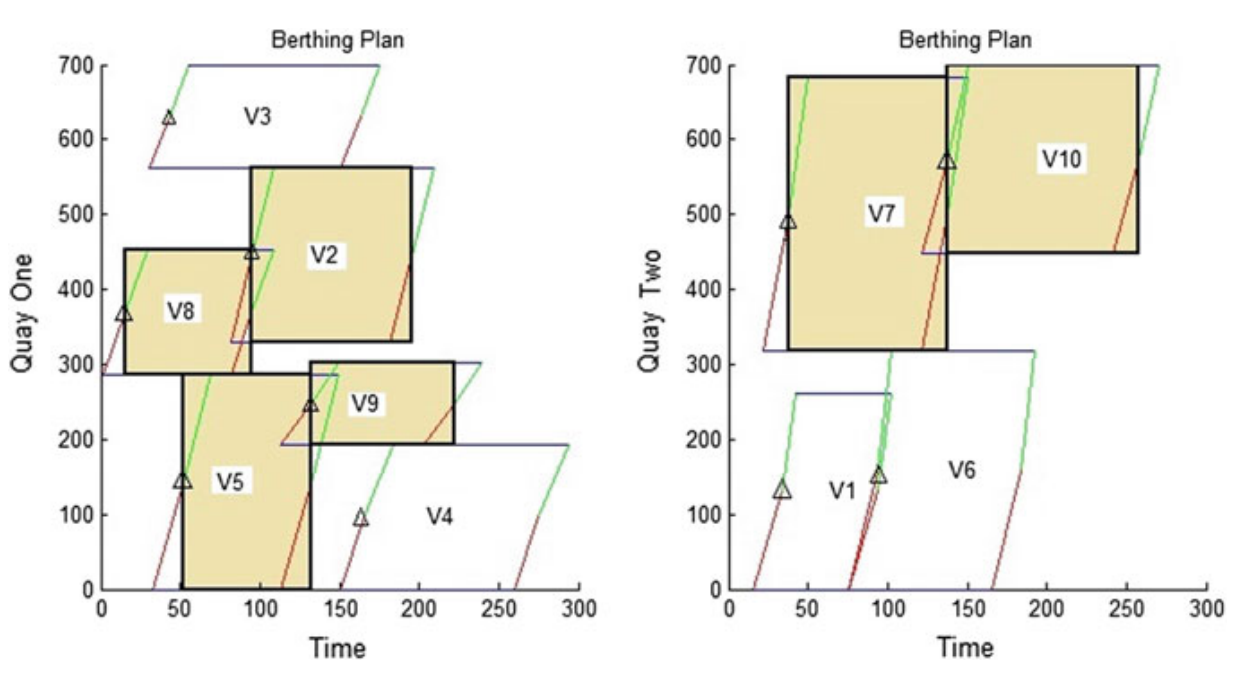
\includegraphics[width=.9\linewidth]{sections/img/bap-example-fuzzy-solution.png}
\caption{\label{fig:bap-example-solution}Example solution of a fuzzy BAP model over multiple quays. The parallelograms represent the fuzzy solution visually by depicting the lower and upper bounds for the arrival and departure times with the vertial sloped lines. The yellow filled squares represent the average crisp solution.}
\end{figure}
\section{The Fuzzy PAP}
\label{sec:the-fuzzy-pap}
This section derives the Fuzzy PAP (FPAP). It is separated into three parts to construct each component individually:
objective function, queuing constraints, and charging constraints. Before deriving the FPAP, it is prudent to define the
set of fuzzy variables. Similarly to the Fuzzy BAP, the arrival times, \(\tilde{a}_i\), berthing time \(\tilde{u}_i\), and
detach time from the charger \(\tilde{d}_i\) are assumed to be imprecise. Thus, indirectly, the service time,
\(\tilde{s}_i\), the linearization constraint in \ref{eq:slack_gain}, \(\tilde{g}_{iq}\), and the initial charge for visit
\(i\), \(\tilde{\eta}_i\) will also become fuzzy values.

\subsection{Objective Function}
\label{sec:orgd02e45c}
Begin by rewriting the crisp objective function with the fuzzy linearization term as shown in \ref{eq:fuzzy-objective}.

\begin{equation}
\label{eq:fuzzy-objective}
\text{min } \sum_{i=1}^{n_I} \sum_{q=1}^{n_Q} \Big( w_{iq} m_q + \tilde{g}_{iq} \epsilon_{q} \Big)
\end{equation}

As shown in \ref{sec:fully-fuzzy-linear-programming}, the method of handling the fuzzy values in the objective function is to
simply apply a ranking function. Let \(\mathfrak{R}\) be defined as the First Index of Yager as shown in \ref{eq:first-index-yager}.
The resulting objective function is shown in \ref{eq:fuzzy-objective-yager}.

\begin{equation}
\label{eq:fuzzy-objective-yager}
\text{min } \sum_{i=1}^{n_I} \sum_{q=1}^{n_Q} \Big( w_{iq} m_q + \mathfrak{R}(g_{iq}) \epsilon_{q} \Big)
\end{equation}

\subsection{Queuing Constraints}
\label{sec:org602fcc5}
To derive the queuing constraints, the set of crisp constraints that are of interest are rewritten in terms of the fuzzy
variables that have been identified prior as shown in \ref{eq:fuzzy-packing-constrs}. \ref{subeq:fp_m_time} fuzzifies all the
temporal terms. \ref{subeq:fp_m_valid_pos} and \ref{subeq:fp_m_sigma} duplicate the constraints \(|\tilde{u}_i|\) times.
Using triangular fuzzy numbers, that would imply constraints for the lower, middle, and upper bounds of the temporal
impreciseness. Similarly, \ref{subeq:fp_m_detach}-\ref{subeq:fp_m_valid_depart} are equivalent to their crisp
counterparts, but with fuzzified terms. \ref{subeq:fp_binaryspace} simply updates the binary decision term.

\begin{multicols}{2}
\begin{subequations} \label{eq:fuzzy-packing-constrs}
\begin{equation}
    \tilde{u}_i - \tilde{u}_j - \tilde{s}_j - (\sigma_{ij} - 1)T \geq 0 \label{subeq:fp_m_time}         \\
\end{equation}
\begin{equation}
    \sigma_{ij} + \sigma_{ji} + \psi_{ij} + \psi_{ji} \geq 1                     \label{subeq:fp_m_valid_pos}    \\
\end{equation}
\begin{equation}
    \sigma_{ij} + \sigma_{ji} \leq 1                                       \label{subeq:fp_m_sigma}        \\
\end{equation}
\begin{equation}
    \tilde{s}_i + \tilde{u}_i = \tilde{d}_i                       \label{subeq:fp_m_detach}       \\
\end{equation}
\begin{equation}
    \tilde{a}_i \leq \tilde{u}_i \leq (T - \tilde{s}_i)                 \label{subeq:fp_m_valid_starts} \\
\end{equation}
\begin{equation}
    \tilde{d}_i \leq \tau_i                                             \label{subeq:fp_m_valid_depart} \\
\end{equation}
\begin{equation}
   \sigma_{ij}, \psi_{ij} \in \{0,1\}\;                                   \label{subeq:fp_binaryspace}        \\
\end{equation}
\end{subequations}
\end{multicols}

\subsection{Charging Constraints}
\label{sec:org1dde3bc}
Similarly to the other derivations, the crisp constraints are rewritten with their equivalent fuzzy terms.
\ref{subeq:fp_init_charge}-\ref{subeq:fp_final_charge} are equivalent to their crisp counterpart with the added lower
and upper bounds for the battery charge for visit \(i\). Note that the discharge amount, \(\Delta_i\), is not fuzzy. It is
assumed that the bus traveled the same distance during the route, thus the same amount of discharge, but can be early,
on time, or late to the station. \ref{subeq:fp_gpgret}-\ref{subeq:fp_gwles} fuzzify the linearization terms in a similar
manner, but the crisp spatial term, \(w_{iq}\) is included. The inclusion of the crisp terms with the fuzzy values is
allowed because although the time may be allowed to fluctuate, the specified queue, discharge amounts, or initial/final
charges are the same for each element of the fuzzy temporal values. Thus, when the fuzzy constraints are converted into
crisp constraints, the constraint validity is maintained \cite{ghanbari-2019-fuzzy}.

\begin{multicols}{2}
\begin{subequations}                                                       \label{eq:fuzzy-dyn-constrs}
\begin{equation}
    \tilde{\eta}_{\Gamma^0_i} = \alpha \kappa_{\Gamma^0_i}                                        \label{subeq:fp_init_charge}    \\
\end{equation}
\begin{equation}
    \tilde{\eta}_i + \sum_{q=1}^{n_Q} \tilde{g}_{iq} r_q - \Delta_i = \tilde{\eta}_{\gamma_i} \label{subeq:fp_next_charge}    \\
\end{equation}
\begin{equation}
    \tilde{\eta}_i + \sum_{q=1}^{n_Q} \tilde{g}_{iq} r_q - \Delta_i \geq \nu \kappa_{\Gamma_i}       \label{subeq:fp_min_charge}     \\
\end{equation}
\begin{equation}
    \tilde{\eta}_i + \sum_{q=1}^{n_Q} \tilde{g}_{iq} r_q \leq \kappa_{\Gamma_i}               \label{subeq:fp_max_charge}     \\
\end{equation}
\begin{equation}
    \tilde{\eta}_{\Gamma^f_i} \geq \beta \kappa_{\Gamma^f_i}                                        \label{subeq:fp_final_charge}   \\
\end{equation}
\begin{equation}
    \tilde{s}_i - (1 - w_{iq})M \leq \tilde{g}_{iq}                           \label{subeq:fp_gpgret}         \\
\end{equation}
\begin{equation}
    \tilde{s}_i \geq \tilde{g}_{iq}                                           \label{subeq:fp_gples}          \\
\end{equation}
\begin{equation}
    Mw_{iq} \geq \tilde{g}_{iq}                                               \label{subeq:fp_gwgret}         \\
\end{equation}
\begin{equation}
    0 \leq \tilde{g}_{iq}                                                     \label{subeq:fp_gwles}          \\
\end{equation}
\end{subequations}
\end{multicols}

\bibliographystyle{plain}
\bibliography{/home/alex/Documents/docs/fuzzy-lp-paper/citation-database/lit-ref,/home/alex/Documents/docs/fuzzy-lp-paper/citation-database/lib-ref,~/Documents/citation-database/lit-ref,~/Documents/citation-database/lib-ref}
\end{document}